In this section, we introduce the problem that we solve.
We first define the problem with particular focus on defining the cost function in a manner that would translate well to the quantum strategy we later employ.
%%%%%%%%%%%%%%%%%%%%%%%%%%%%%%%%%%%
\section{The Max Cut problem}
Consider an unweighted un-directional graph $G := (V, E)$. $V$ is the set of vertices (or nodes) of the graph while $E$ is the set of edges.
Consider a partition of the vertices into two disjoint subsets, namely, set $A$ and set $B$.
Any general partition of the vertices will potentially have edges such that the two nodes at the end of the edge are in different subsets.
Thus, the partition boundary can be said to have \textit{cut} the edge.
Let the number of edges being cut by a partition $i$ be $C_i$.
The \textbf{MaxCut} problem is to find the partition for any given graph $G$ such that the $C_i$ is maximum.
Thus, we want to find the partition that crosses the maximum number of edges.

It is instructive to look at the nature of the problem and the solution space here.
The problem is to optimize a certain function (number of edges being crosses by the partition) under certain conditions (the graph G).
One partition varies from other partition in terms of the combination of nodes chosen to be together in one subset.
Thus, the solution space is all possible partitions, which are all possible combinations of the nodes.
This means, the solution space is discrete.
Problems of this kind are called \textit{combinatorial optimization problem}.

The discrete solution space grows extremely rapidly with the size of the graph that we consider.
The solution space grows as $\mathcal{O}(2^n)$ where $n$ is the number of nodes in the graph.
Thus, for large graphs, the simplest solution, that is, checking all partitions is very costly.
There are other better classical algorithms but the problem remains very difficult and costly to solve.
In fact, MaxCut is an NP-Hard problem. Thus finding a solution for a general graph G is not possible.
Approximate algorithms that run in polynomial time do however exist.

%%%%%%%%%%%%%%%%%%%%%%%%%%%%%%%%%%%
\section{Mathematical Formulation}

Let us define a function that identifies which subset any particular node is in. We define a function
\begin{equation}
     g(i) = \begin{cases} 
         1 & i \in A \\
        -1 & i \in B 
   \end{cases}
   \label{g_def}
\end{equation}
Thus, for any edge with vertices $i$ and $j$, if it is being cut by the partition or not can be given by
\begin{equation}
    C_{ij} = \frac{1}{2}(1 - g(i)g(j))
    \label{C_def}
\end{equation}
Consequentially, the total number of edges being cut is simply the sum of $C_{ij}$ over all edges. Thus, the function that we want to maximize is

$$C(g) = \sum_{(i, j) \in E}C_{ij} = \frac{1}{2}\sum_{(i, j) \in E}(1 - g(i)g(j))$$

Here, $g$ can be seen as a string of length n where the $g_i = g(i)$.
We will use this idea when we implement the quantum algorithm.

\begin{figure}[h]
    \centering
    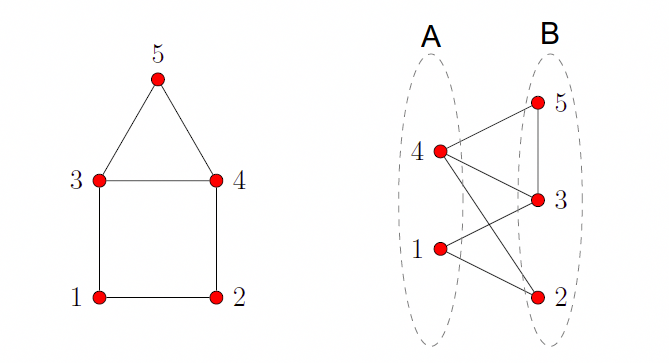
\includegraphics[scale=0.65]{images/GraphCut.png}
    \caption{A 5 node graph with one possible partition of the nodes.}
    \label{fig:GraphCut}
\end{figure}

As an illustration, let us consider a 5 node graph with the connectivity as shown in the figure \ref{fig:GraphCut} above.
Additionally, say we have the partition in two sets, namely $A$ and $B$ as shown in the figure.
For this particular partition, the number of edges being cut are 5.
Note that, for any partition, there exists another partition with all the nodes between the two exchanged.
These two partitions would have the same number of edges being cut.

Having established the problem, next we look at the algorithm to solve it.